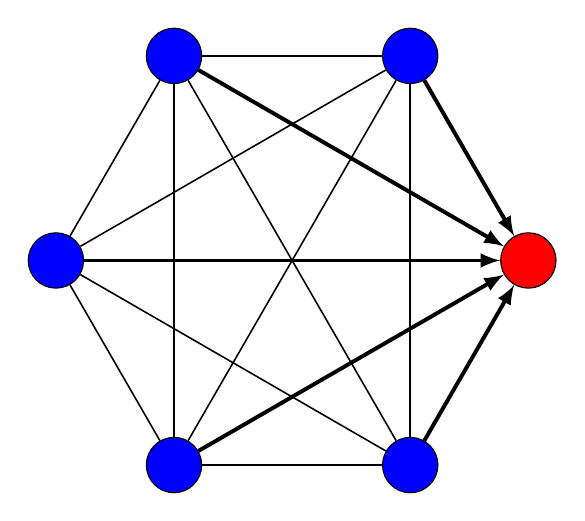
\begin{tikzpicture}
    \foreach \i in {1,...,6} {
        \ifnum\i=1
            \node[draw, fill=red, circle, minimum size=20pt] (v\i) at ({360/6 * (\i-1)}:3) {};
        \else
            \node[draw, fill=blue, circle, minimum size=20pt] (v\i) at ({360/6 * (\i-1)}:3) {};
        \fi
    }
    
    \foreach \i in {1,...,6} {
        \foreach \j in {1,...,6} {
            \ifnum\i<\j
                \ifnum\i=1
                    \draw[->, line width=0.5mm, >=latex] (v\j) -- (v\i);
                \else
                    \draw[line width=0.2mm] (v\i) -- (v\j);
                \fi
            \fi
        }
    }
\end{tikzpicture}